\title{Lecture 12: Probability in Board Games and Complex Numbers}

\frame{\titlepage}

%%%%%%%%%%%%%
\section[Expected]{Advanced Expected Value}
\frame{\sectionpage}
%%%%%%%%%%%%%

\begin{frame}{Infinite Sum}
The formula for expected value still works if there are infinitely many outcomes. The following formula for geometric series might be useful:
\begin{block}{Geometric series sum}
If $-1 < r < 1$, then
\[ \sum_{n=0}^{\infty} r^n = 1 + r + r^2 + r^3 + \ldots = \frac{1}{1-r}.\]
\end{block}
\end{frame}
\begin{frame}[t]{Geometric series: a positive ratio}
\small
\begin{ex}
Find $1+\frac13+\frac19+\frac1{27}+\cdots$.
\end{ex}
\begin{sol}
The common ratio is $r=1/3$, and $|r|<1$. Thus\[\sum_{n=0}^{\infty}\left(\frac13\right)^n=\frac{1}{1-1/3}=\frac32.\] The initial term $1$ corresponds to $n=0$.
\end{sol}
\end{frame}

\begin{frame}[t]{Geometric series: alternating signs}
\small
\begin{ex}
Find $1-\frac12+\frac14-\frac18+\cdots$.
\end{ex}
\begin{sol}
Here $r=-1/2$, still with $|r|<1$. Therefore\[\sum_{n=0}^{\infty}\left(-\frac12\right)^n=\frac{1}{1-(-1/2)}=\frac23.\] The formula permits negative ratios, as long as their absolute value is less than one.
\end{sol}
\end{frame}



\begin{frame}[t]
\begin{ex}
Suppose you flip a coin until you see a tail. What is the expected number of flips?
\end{ex}
\begin{sol}
Let $X$ be the number of coin flips until we get a tail. For $X = k$, there must be $k-1$ consecutive heads, and then 1 last tail. Since each flip is independent, the probability is $\frac{1}{2^k}$. Hence,
\begin{eq*}
\red{E(X)} &=& \sum_{x = 1}^{\infty} x P(X=x) = \sum_{x=1}^{\infty} \frac{x}{2^x} =\frac{1}{2} + \frac{2}{4} + \frac{3}{8} + \frac{4}{16} + \ldots \\
\green{2E(X)} &=& 1 + \frac{2}{2} + \frac{3}{4} + \frac{4}{8} + \frac{5}{16} + \ldots \\
\green{2E(X)} -\red{E(X)} &=& 1 + \frac{1}{2} + \frac{1}{4} + \frac{1}{8} + \frac{1}{16} + \ldots \\
E(X) &=& 2
\end{eq*}
Thus, on average, we need to flip 2 times to see the first tail.
\end{sol}
\end{frame}

\begin{frame}
\frametitle{Recursive Formula}
It is possible that a formula of $E(X)$ contains the term $E(X)$ itself! This happens when there is a case when the experiment must be repeated.
\end{frame}


\begin{frame}[t]
\begin{ex}
Suppose you flip a coin until you see a tail. What is the expected number of flips?
\end{ex}
\begin{sol}
Let $X$ be the number of coin flips until we get a tail. 
\begin{itemize}
\item On a tail, the experiment ends and the number of flips is 1. 
\item On a head, the experiment is repeated, and the number of flips is $E(X) + 1$.
\end{itemize}
Thus, we have
\begin{eq*}
E(X) &=& (1) \frac{1}{2} + (E(X) + 1) \frac{1}{2} \\
E(X) &=& 1 + \frac{E(X)}{2} \\
E(X) &=& 2
\end{eq*}
This gives the same result as before.
\end{sol}
\end{frame}


\begin{frame}[t]
\begin{ex}
Suppose you roll a die. If the result is less than 6, you get that many coins. If the result is 6, you must pay a penalty of 5 coins before rerolling again. What is the expected number of coins you would gain?
\end{ex}
\begin{sol}
Let $X$ be the amount of coins you gain. There is $\tfrac{1}{6}$ chance to roll a 1 and get 1 coin. There is $\tfrac{1}{6}$ chance to roll a 2 and get 2 coins, and so on. Finally, there is $\tfrac{1}{6}$ chance to roll a 6 and get $E(X) - 5$ coins. Thus, we have
\begin{eq*}
E(X) &=& (1) \frac{1}{6} + (2) \frac{1}{6} + (3) \frac{1}{6} + (4) \frac{1}{6} + (5) \frac{1}{6} + (E(X)-5) \frac{1}{6} \\
E(X) &=& \frac{10}{6} + \frac{E(X)}{6} \\
E(X) &=& 2
\end{eq*}
Thus, despite the penalty on rolling 6, on average you still gain 2 coins!
\end{sol}
\end{frame}

\begin{frame}[t]{Waiting for two consecutive heads}
\small
\begin{ex}
Flip a fair coin independently until two consecutive heads first appear.
Starting before any flips, what is the expected number of flips?
\end{ex}
\begin{sol}
We need two states, depending on the most recent flip:
\begin{itemize}
\item $E_0$: expected remaining flips when starting, or after a tail.
\item $E_H$: expected remaining flips when the last flip was a head,
but we have not yet obtained HH.
\end{itemize}
Count the next flip first, then the remaining waiting time:
\[
E_0=1+\tfrac12 E_0+\tfrac12 E_H,\qquad
E_H=1+\tfrac12 E_0+\tfrac12(0).
\]
From state H, another head finishes; a tail returns us to state $0$.
\end{sol}
\end{frame}

\begin{frame}[t]{Two consecutive heads: solve the recurrence}
\begin{sol}
Substitute $E_H=1+\tfrac12 E_0$ into the equation for $E_0$:
\begin{align*}
E_0&=1+\tfrac12 E_0+\tfrac12\left(1+\tfrac12 E_0\right)\\
   &=\tfrac32+\tfrac34 E_0,\\
\tfrac14 E_0&=\tfrac32,\qquad E_0=6.
\end{align*}
Thus, starting from scratch, the expected waiting time is
\[
\boxed{6\text{ flips}}.
\]
If the last flip was already H, the expected remaining time is
$E_H=1+\tfrac12(6)=4$ flips.
\end{sol}
\end{frame}

%%%%%%%%%%%%%%%%%%
\section[Dice]{Complex Dice Example}
\frame{\sectionpage}
%%%%%%%%%%%%%%%%%%

\begin{frame}{Risk}
\begin{itemize}
\item Attacker and Defender roll some dice. 
\item Sort dice on each side from highest to lowest.
\item Compare highest pair of dice. The smaller value loses 1 troop; when tied, the attacker loses 1 troop.
\end{itemize}
\end{frame}


\begin{frame}
\addfig{0.8}{dice_risk.png}{Dice combat in Risk}
\end{frame}

\begin{frame}[t]
\begin{ex}
If attacker and defender each roll a single die, find the expected win for the attacker.
\end{ex}
\begin{sol}
Create a table listing all possible outcomes.
\begin{figure}[h!]
\centering
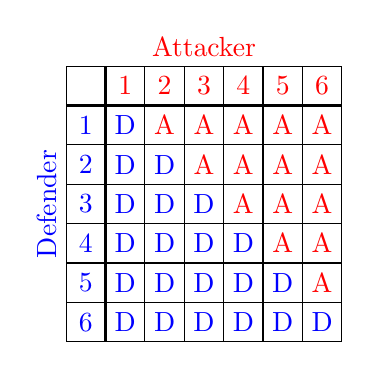
\begin{tikzpicture}[scale = 0.5, yscale = -1]
\draw (0,0) grid (7,7);
\draw[very thick] (1,0) -- (1,7) (0,1) -- (7,1);
\begin{scope}[xshift = 0.5cm, yshift = 0.5cm]
\node[red] at (3,-1) {Attacker};
\node[blue, rotate = 90] at (-1,3) {Defender};
\foreach \x in {1,2,3,4,5,6}
{
\node[red] at (\x, 0) {$\x$};
\node[blue] at (0, \x) {$\x$};
}
\foreach \attack in {1,2,3,4,5,6}
{
	\foreach \defend in {1,2,3,4,5,6}
	{
		\ifnum\attack > \defend
			\node[red] at (\attack, \defend) {A};
		\else
			\node[blue] at (\attack, \defend) {D};
		\fi 
	}
}
\end{scope}
\end{tikzpicture}
\end{figure}
We see that the attacker wins 15 out of 36 equally likely outcomes. Therefore, the expected win is $E(X) = \tfrac{15}{36} = \tfrac{5}{12}$ for each combat.
\end{sol}
\end{frame}

\begin{frame}[t]
\begin{ex}
If attacker rolls two dice and defender rolls one die, find the expected win for the attacker.
\end{ex}
\begin{sol}
First, let $X$ be the maximum of two dice for the attacker and determine $P(X)$ for each possible value. 
\begin{figure}[h!]
\centering
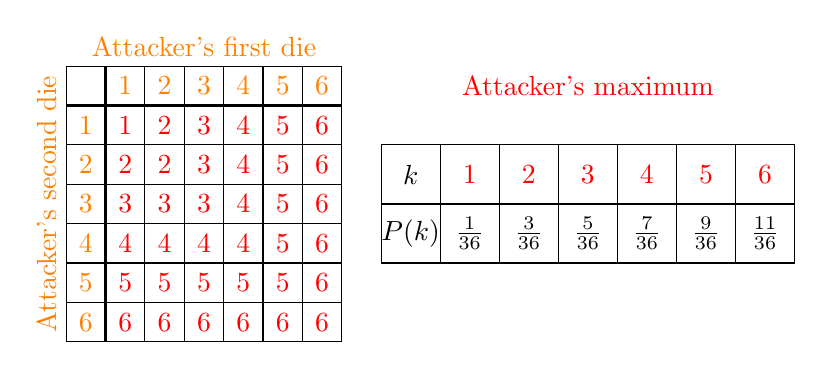
\begin{tikzpicture}[scale = 0.5, yscale = -1]
\draw (0,0) grid (7,7);
\draw[very thick] (1,0) -- (1,7) (0,1) -- (7,1);
\begin{scope}[xshift = 0.5cm, yshift = 0.5cm]
\node[orange] at (3,-1) {Attacker's first die};
\node[orange, rotate = 90] at (-1,3) {Attacker's second die};
\foreach \x in {1,2,3,4,5,6}
{
\node[orange] at (\x, 0) {$\x$};
\node[orange] at (0, \x) {$\x$};
}
\foreach \first in {1,2,3,4,5,6}
{
	\foreach \second in {1,2,3,4,5,6}
	{
		\ifnum\first > \second
			\node[red] at (\first, \second) {\first};
		\else
			\node[red] at (\first, \second) {\second};
		\fi 
	}
}
\end{scope}
% table on the right
\begin{scope}[xshift = 8cm, yshift = 2cm, scale = 1.5]
\draw (0,0) grid (7,2);
\node[red] at (3.5, -1) {Attacker's maximum};
\begin{scope}[xshift = 0.5cm, yshift = 0.5cm]
\node at (0,0) {$k$};
\node at (0,1) {$P(k)$};
\foreach \x /\p in {1/1,2/3,3/5,4/7,5/9,6/11}
{
\node[red] at (\x, 0) {$\x$};
\node at (\x,1) {$\frac{\p}{36}$};
}
\end{scope}
\end{scope}
\end{tikzpicture}
\label{}
\end{figure}
\end{sol}
\end{frame}

\begin{frame}[t]
\begin{sol} (Continued)
Then, we can apply these values to the previous table, but replacing a single win (A) with the actual probability from the second table.
\begin{figure}[h!]
\centering
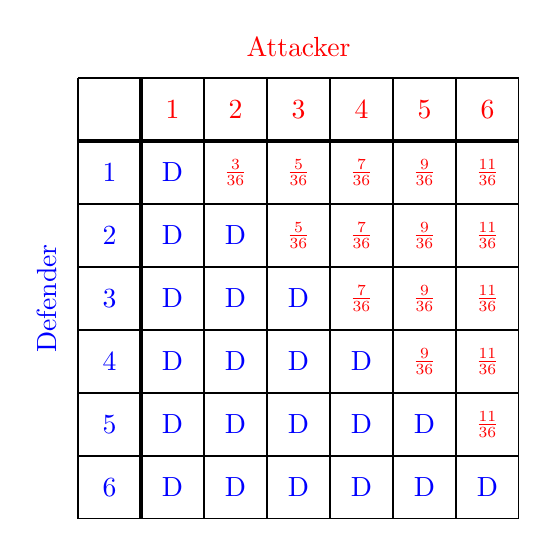
\begin{tikzpicture}[scale = 0.8, yscale = -1]
\draw (0,0) grid (7,7);
\draw[very thick] (1,0) -- (1,7) (0,1) -- (7,1);
\begin{scope}[xshift = 0.5cm, yshift = 0.5cm]
\node[red] at (3,-1) {Attacker};
\node[blue, rotate = 90] at (-1,3) {Defender};
\foreach \x in {1,2,3,4,5,6}
{
\node[red] at (\x, 0) {$\x$};
\node[blue] at (0, \x) {$\x$};
}
\foreach \attack / \p in {1/1,2/3,3/5,4/7,5/9,6/11}
{
	\foreach \defend in {1,2,3,4,5,6}
	{
		\ifnum\attack > \defend
			\node[red, scale = 0.8] at (\attack, \defend) {$\frac{\p}{36}$};
		\else
			\node[blue] at (\attack, \defend) {D};
		\fi 
	}
}
\end{scope}
\end{tikzpicture}
\end{figure}
\end{sol}
\end{frame}

\begin{frame}
\begin{sol} (Continued)
Here is how to interpret the table: in the first row when the defender rolls a 1, the attacker wins if they roll 2,3,4,5 or 6. Thus, the total in that case is $\frac{3}{36} + \frac{5}{36} + \frac{7}{36} + \frac{9}{36} + \frac{11}{36} = \frac{35}{36}$. 

\begin{figure}[h!]
\centering
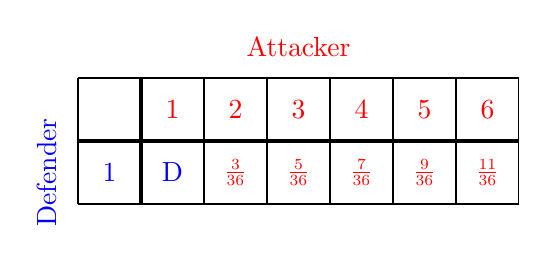
\begin{tikzpicture}[scale = 0.8, yscale = -1]
\draw (0,0) grid (7,2);
\draw[very thick] (1,0) -- (1,2) (0,1) -- (7,1);
\begin{scope}[xshift = 0.5cm, yshift = 0.5cm]
\node[red] at (3,-1) {Attacker};
\node[blue, rotate = 90] at (-1,1) {Defender};
\foreach \x in {1,2,3,4,5,6}
{
\node[red] at (\x, 0) {$\x$};
}
\node[blue] at (0,1) {1};
\foreach \attack / \p in {1/1,2/3,3/5,4/7,5/9,6/11}
{
	\ifnum\attack > 1
		\node[red, scale = 0.8] at (\attack, 1) {$\frac{\p}{36}$};
	\else
		\node[blue] at (\attack, 1) {D};
	\fi 
}
\end{scope}
\end{tikzpicture}
\end{figure}

Since the defender's values from 1-6 are equally likely, the expected number can be obtained by adding all red numbers:
\[ E(X) = \frac{1}{6}\left(\frac{35}{36} + \frac{32}{36} + \frac{27}{36} + \frac{20}{36} + \frac{11}{36}\right) = \frac{125}{216}.\]
\end{sol}
\end{frame}

\begin{frame}{Yahtzee}
Roll 5 dice. You can keep any number of dice and reroll the rest. Then, you can keep any number of dice (either previously rerolled or not), and reroll the rest. Then the result is compared to a poker-hand-like table.
\end{frame}

\begin{frame}{}
\addfig{0.7}{dice_yahtzee}{Dice hand in Yahtzee}
\end{frame}

\begin{frame}[t]
\begin{ex}
Find the probability of getting a Yahtzee if you are allowed to reroll once (with any number of dice).
\end{ex}
\begin{sol}
\begin{itemize}
\item If our very first roll gives us a Yahtzee already, we win, with probability $\frac{6}{6^5}$.
\item If the first roll is four-of-a-kind, then we reroll the last die. The probability of getting four-of-a-kind is 
\[\frac{6 \times C(5,4) \times 5}{6^5} = \frac{150}{6^5}.\] 
We first consider which value is the four-of-a-kind (6 possibilities), then which die is the fifth unmatched die ($\binom{5}{4}$), and lastly which value is on the fifth die (5 possibilities).
\end{itemize}
\end{sol}
\end{frame}

\begin{frame}
\begin{sol} (Continued)
Therefore, the probability of getting a four-of-a-kind and then rerolling to get a Yahtzee is 
\[\frac{150}{6^5} \times \frac{1}{6} = \frac{25}{6^5}.\]
\begin{itemize}
\item If the first roll has three matching values, we apply a similar argument. The probability of getting such outcome is 
\[\frac{6 \times C(5,3) \times (5 \times 5)}{6^5} = \frac{1500}{6^5}.\] 
Then, the probability of rerolling two dice to match the first three is $\frac{1}{36}$. Thus, the probability is 
\[\frac{1500}{6^5} \times \frac{1}{36} = \frac{250}{6^6}.\]
\end{itemize}
\end{sol}
\end{frame}

\begin{frame}{Can't Stop: choose how to pair four dice}
\small
\begin{itemize}
\item Roll four dice and split them into two pairs. Each pair's sum
selects a numbered column in which to advance a runner.
\item At most three columns can be active during a turn. After a
successful roll, stop to bank progress or roll again and risk losing it.
\item Complete three columns to win.
\end{itemize}
For the roll $(2,3,4,5)$, the three pairings give:
\begin{center}
\begin{tabular}{c|c}
Pairing & Column totals \\
\hline
$(2,3)$ and $(4,5)$ & $5$ and $9$ \\
$(2,4)$ and $(3,5)$ & $6$ and $8$ \\
$(2,5)$ and $(3,4)$ & $7$ and $7$
\end{tabular}
\end{center}
Two pairs totaling $7$ can advance that runner twice, if there is room.

\medskip
{\footnotesize\href{https://en.boardgamearena.com/gamepanel?game=cantstop}{Rules reference: Board Game Arena, Can't Stop}}
\end{frame}

\begin{frame}[t]{Can't Stop: first, can we advance on 2?}
\small
\begin{ex}
A runner is on column $2$ and has room to advance.
Roll four independent fair six-sided dice. What is the probability
that some pairing lets you advance this runner at least once?
\end{ex}
\begin{sol}
The only pair totaling $2$ is $1+1$, so we need \textbf{at least two ones}.
Count the complementary cases among the $6^4=1296$ ordered rolls:
\[
\underbrace{5^4=625}_{\text{no ones}},\qquad
\underbrace{4\cdot5^3=500}_{\text{exactly one one}}.
\]
For exactly one one, choose its die in $4$ ways; the other three dice
each have $5$ choices, namely $2,3,4,5,6$.
\[
P(\text{can advance on }2)
=1-\frac{625+500}{1296}
=\boxed{\frac{19}{144}\approx13.19\%}.
\]
Rolls with three or four ones are successful too; count each roll once.
\end{sol}
\end{frame}

\begin{frame}[t]{Can't Stop example: can we advance on 7?}
\small
\begin{ex}
A runner is already on column $7$ and has room to advance.
Roll four independent fair six-sided dice. What is the probability
that some pairing lets you advance this runner at least once?
\end{ex}
\begin{sol}
There are $6^4=1296$ equally likely ordered rolls. A pair totals $7$
exactly when it uses one of these complementary face pairs:
\[
\{1,6\},\qquad\{2,5\},\qquad\{3,4\}.
\]
Let $A_{16}$ mean that both a $1$ and a $6$ occur; define $A_{25}$
and $A_{34}$ similarly. We want their union.

\end{sol}
\end{frame}

\begin{frame}[t]{Can't Stop: count one complementary face pair}
\small
\begin{sol}
To find $|A_{16}|$, start with all ordered rolls:
\begin{itemize}
\item All four dice are unrestricted: $6^4$ rolls.
\item No die shows $1$: $5^4$ rolls.
\item No die shows $6$: $5^4$ rolls.
\item Neither $1$ nor $6$ appears: $4^4$ rolls.
\end{itemize}
For $A_{16}$, subtract rolls with no $1$ or no $6$, then restore
rolls with neither:
\[
|A_{16}|=6^4-2\cdot5^4+4^4=302.
\]
The same count applies to $A_{25}$ and $A_{34}$.
\end{sol}
\end{frame}

\begin{frame}[t]{Can't Stop: correct for overlapping possibilities}
\small
\begin{sol}
A roll in $A_{16}\cap A_{25}$ must contain $1,6,2,5$, each once.
These can be ordered in $4!=24$ ways.

\medskip
Each of the three pairwise intersections has $24$ rolls. The triple
intersection is impossible: it would require six distinct faces on four dice.
By inclusion-exclusion,
\begin{align*}
|A_{16}\cup A_{25}\cup A_{34}|
 &=3(302)-3(24)=834,\\
P(\text{can advance on }7)
 &=\frac{834}{1296}=\boxed{\frac{139}{216}\approx64.35\%}.
\end{align*}
Count each roll once, even if it has several usable pairings.
Other active columns can also provide moves on a roll that cannot make $7$.
\end{sol}
\end{frame}

%%%%%%%%%%%%%%%%%%
\section{Complex Numbers}
\frame{\sectionpage}
%%%%%%%%%%%%%%%%%%

% Section: Motivation
\begin{frame}{Intuition}
  \begin{itemize}
    \item Complex numbers appear in physics, engineering, and computer graphics.
    \item They let us solve equations that have no real solutions (e.g., $x^2+1=0$).
    \item Learning them builds algebra and geometric intuition.
  \end{itemize}
\end{frame}

\begin{frame}{Integers}
  \begin{itemize}
  \item First we have the set of natural numbers 
  \[\mathbb{N} =\{1,2,3,\ldots\}.\]
  \item Adding two natural numbers (say $3+9$) results in another natural number. This property is called closed: the set of natural numbers is closed under addition (and also multiplication).
  \item But subtracting one natural number from another does not always give you another natural number (say $5-8$).
  \item Fix: define negative numbers. Now we have the set of integers 
  \[\mathbb{Z} = \{\ldots, -2,-1,0,1,2,\ldots\}.\]
  \end{itemize}
\end{frame}

\begin{frame}{Fractions}
  \begin{itemize}
  \item Great! Now adding, multiplying, or subtracting two integers gives you another integer.
  \item But now division doesn't work!
  \item Fix: define fractions. Now we have the set of rational numbers 
  \[\mathbb{Q} = \left\{\frac{a}{b} \Big| a,b \in \mathbb{Z}, b \neq 0 \right\}.\]
  \end{itemize}
\end{frame}

\begin{frame}{Real Numbers}
  \begin{itemize}
  \item Great! Now adding, subtracting, multiplying, or dividing rational numbers gives another rational number.
  \item But the system is still flawed! There are numbers that can't be represented as a fraction of two integers, like the length of the hypotenuse of a right triangle with side lengths 1, or the circumference of a circle with radius 1.
  \begin{figure}[h!]
  \centering
  \begin{tikzpicture}[scale = 0.6]
  \begin{scope}[xshift =2cm]
  \draw (0,0) -- (2,0) node[pos=0.5, below] {$1$};
  \draw (2,0) -- (2,2) node[pos=0.5, right] {$1$};
  \draw (2,2) -- (0,0) node[pos=0.5, above left] {$?$};
  \end{scope}
  \draw[->] (0,1.1) arc[start angle = 0, end angle = 355, radius = 0.6] node[pos=0.5, left] {$?$};
  \end{tikzpicture}
  \end{figure}
  \item Fix: define real numbers. Now we have the set of real numbers:
\[\mathbb{R} = \left\{ x \, \Big| x \text{ can be written as a decimal number.}\right\} \]
$\sqrt{2}$ and $\pi$ are real numbers because we can write $\sqrt{2} = 1.41421356\ldots$ and $\pi = 3.14159265\ldots$
  \end{itemize}
\end{frame}

\begin{frame}{Here comes the complex numbers}
  \begin{itemize}
  \item Great! Now we have all these fancy numbers!
  \item But the system is still flawed! Polynomials like
  \[x^2+1 = 0\]
  do not have solutions in real numbers.
  \item Fix: assume they have solutions, which we define as ``complex numbers''. Now we have the set of complex numbers $\mathbb{C}$.
  \end{itemize}
\end{frame}

\begin{frame}{The imaginary unit $i$}
\begin{thm}{}{}
Let $i$ be a root of the polynomial
\[x^2+1=0\]
\end{thm}
  \begin{itemize}
    \item We see that \(i^2 = -1.\)
    \item This seems strange because no real number squared gives $-1$.
    \item But we can treat $i$ as a new number that expands our number system.
  \end{itemize}
\end{frame}
\begin{frame}[t]{Imaginary unit: squaring a multiple}
\small
\begin{ex}
Compute $(2i)^2$ using $i^2=-1$.
\end{ex}
\begin{sol}
\[(2i)^2=4i^2=4(-1)=-4.\] A purely imaginary number can have a negative real square.
\end{sol}
\end{frame}

\begin{frame}[t]{Imaginary unit: solving an equation}
\small
\begin{ex}
Solve $z^2+9=0$ over the complex numbers.
\end{ex}
\begin{sol}
\[z^2=-9\quad\Longrightarrow\quad z=3i\text{ or }z=-3i.\] Both roots satisfy $(\pm3i)^2=9i^2=-9$. There are no real roots.
\end{sol}
\end{frame}


\begin{frame}{Notation: Complex numbers}
  \begin{defn}{}{}
A \textbf{complex number} has the form 
\begin{equation}
z = a + bi,
\end{equation}
where $a$ and $b$ are real numbers.

\tcblower
$a$ is called the \textbf{real part} (\(\Re(z)=a\)), and $b$ is the \textbf{imaginary part} (\(\Im(z)=b\)).
\end{defn}
\end{frame}


\begin{frame}{Addition and subtraction}
\begin{thm}{}{}
Let $a+bi$ and $c+di$ be complex numbers. 
\begin{eq}
(a+bi) + (c+di) &=& (a + c) + (b + d)i \\
(a+bi) - (c+di) &=& (a - c) + (b - d)i
\end{eq}
\end{thm}
\end{frame}

\begin{frame}[t]
\begin{ex}
Compute the following additions.
\begin{tasks}(3)
\task $(3+2i) + (4-5i)$
\task $(4i) + (-2+3i)$
\task $(-1-i) + 5$
\end{tasks}
\end{ex}
\begin{sol}
\begin{tasks}(1)
\task $(3+2i) + (4-5i) = (3+4) + (2-5)i = 7-3i$
\task $(4i) + (-2+3i) = (0+(-2)) + (4+3)i = -2+7i$
\task $(-1-i) + 5 = (-1+5) + (-1+0)i = 4-i$
\end{tasks}
\end{sol}
\end{frame}

\begin{frame}[t]
\begin{ex}
Compute the following subtractions.
\begin{tasks}(3)
\task $(3+2i) - (4-5i)$
\task $(4i) - (-2+3i)$
\task $(-1-i) - 5$
\end{tasks}
\end{ex}
\begin{sol}
\begin{tasks}(1)
\task $(3+2i) - (4-5i) = (3-4) + (2-(-5))i = -1+7i$
\task $(4i) - (-2+3i) = (0-(-2)) + (4-3)i = 2+i$
\task $(-1-i) - 5 = (-1-5) + (-1-0)i = -6-i$
\end{tasks}
\end{sol}
\end{frame}

\begin{frame}{Multiplication}
Multiply like polynomials and use $i^2=-1$:
\begin{eq*}
(a+bi)(c+di) &=& ac + a(di) + (bi)c + (bi)(di) \\
&=& ac + (ad)i + (bc)i + bd(i^2) \\
&=& ac + (ad)i + (bc)i - bd \\
&=& (ac-bd) + (ad+bc)i
\end{eq*}
  \begin{thm}{}{}
    \begin{equation} 
    (a+bi)(c+di) = (ac - bd) + (ad+bc)i
    \end{equation}
  \end{thm}
Note: do not memorize the formula! You should multiply complex numbers like polynomials.
\end{frame}


\begin{frame}[t]
\begin{ex}
Compute the following products.
\begin{tasks}(3)
\task $(3+2i)(4-5i)$
\task $(4i)(-2+3i)$
\task $(5)(-1-i)$
\end{tasks}
\end{ex}
\begin{sol}
\begin{eq*}
(3+2i)(4-5i) &=& (3)(4) + (3)(-5i) + (2i)(4) + (2i)(-5i) \\
&=& 12 - 15i + 8i - 10(-1) \\
&=& 12 - 7i + 10 = 22 - 7i \\
(4i)(-2+3i) &=& (4i)(-2) + (4i)(3i)\\
 &=& -8i - 12 \\
 &=& -12 - 8i \\
(5)(-1-i) &=& (5)(-1) + (5)(-i) \\
&=& -5-5i
\end{eq*}
\end{sol}
\end{frame}

\begin{frame}{Conjugate}
\begin{defn}{}{}
Complex conjugation is denoted with a bar and defined by
\begin{equation}
\overline{a+bi} = a-bi
\end{equation}
If $z=a+bi$, then its conjugate is $\overline{z} = a-bi$ and we read this as ``z-bar''  
\end{defn}

The complex conjugation has a useful property: if $z = a+bi$, then
\[z\overline{z} = (a+bi)(a-bi) = a^2 - (bi)^2 = a^2+b^2,\]
which has no imaginary part.
\end{frame}
\begin{frame}[t]{Conjugate product: a complex pair}
\small
\begin{ex}
Let $z=1+2i$. Compute $z\overline z$ and its modulus.
\end{ex}
\begin{sol}
\[\overline z=1-2i,\quad z\overline z=(1+2i)(1-2i)=1-(2i)^2=5.\] Hence $|z|=\sqrt5$ and $z\overline z=|z|^2$, a nonnegative real number.
\end{sol}
\end{frame}

\begin{frame}[t]{Conjugate product: a negative real part}
\small
\begin{ex}
Let $w=-3+4i$. Compute $w\overline w$ and its modulus.
\end{ex}
\begin{sol}
\[\overline w=-3-4i,\quad w\overline w=(-3)^2+4^2=25.\] Thus $|w|=5$. A negative real part does not make the conjugate product negative.
\end{sol}
\end{frame}


\begin{frame}[t]
\begin{ex}
Find the complex conjugations of the following complex numbers.
\begin{tasks}(4)
\task $2+6i$
\task $-4-3i$
\task $8i$
\task $-7$
\end{tasks}
\end{ex}
\begin{sol}
\begin{tasks}(1)
\task $\overline{2+6i}=2-6i$
\task $\overline{-4-3i} = -4+3i$
\task $\overline{8i} = -8i$
\task $\overline{-7} = -7$
\end{tasks}
\end{sol}
\end{frame}

\begin{frame}{Division}
To divide, the denominator must be nonzero. Multiply numerator and denominator by the \textbf{conjugate} of the denominator.
\begin{thm}{}{}
\begin{equation}
\frac{a+bi}{c+di} = \frac{(a+bi)(c-di)}{(c+di)(c-di)} = \frac{(ac+bd) + (bc-ad)i}{c^2+d^2}
\end{equation}
\end{thm}
Again, do not remember this formula.
\end{frame}
\begin{frame}[t]{Complex division: both parts nonzero}
\small
\begin{ex}
Write $\dfrac{3+2i}{1-i}$ in rectangular form.
\end{ex}
\begin{sol}
Multiply by the denominator conjugate:\[\frac{3+2i}{1-i}=\frac{(3+2i)(1+i)}{(1-i)(1+i)}=\frac{1+5i}{2}=\frac12+\frac52i.\] The denominator is $1^2+(-1)^2=2$.
\end{sol}
\end{frame}

\begin{frame}[t]{Complex division: imaginary denominator}
\small
\begin{ex}
Write $\dfrac{4-2i}{2i}$ in rectangular form.
\end{ex}
\begin{sol}
The denominator conjugate is $-2i$:\[\frac{4-2i}{2i}=\frac{(4-2i)(-2i)}{(2i)(-2i)}=\frac{-4-8i}{4}=-1-2i.\] Check that $(2i)(-1-2i)=4-2i$.
\end{sol}
\end{frame}
\begin{frame}[t]{Division example: recover an unknown factor}
\begin{ex}
A complex number $z$ satisfies $(1+i)z=3-i$. Find $z$ in rectangular form.
\end{ex}
\begin{sol}
Divide by $1+i\ne0$ and multiply by its conjugate:
\begin{align*}
z&=\frac{3-i}{1+i}
  =\frac{(3-i)(1-i)}{(1+i)(1-i)}\\
 &=\frac{3-3i-i+i^2}{1-i^2}
  =\frac{2-4i}{2}=1-2i.
\end{align*}
Check: $(1+i)(1-2i)=3-i$.
\end{sol}
\end{frame}



%%%%%%%%%%%%%%%%
\section[Plane]{Complex plane}
\frame{\sectionpage}
%%%%%%%%%%%%%%%%

\begin{frame}{Complex plane and rectangular form}
  \begin{columns}
    \column{0.4\textwidth}
      We can picture complex numbers on a plane: horizontal axis for the real part, vertical axis for the imaginary part.
      \begin{itemize}
        \item Point $(a,b)$ corresponds to $a+bi$.
        \item Example: $3-2i$ is the point $(3,-2)$.
      \end{itemize}
     We will call $a+bi$ a \text{rectangular form}, because $a$ and $b$ represent rectangle's width and height.
    \column{0.6\textwidth}
      \begin{center}
      \begin{tikzpicture}[scale=0.8]
        \draw[<->] (-3.5,0) -- (3.5,0) node[right]{Re};
        \draw[<->] (0,-3.5) -- (0,3.5) node[above]{Im};
        \foreach \x in {-3,-2,-1,1,2,3} \draw (\x,0.05)--(\x,-0.05) node[below=2pt]{\small\x};
        \foreach \y in {-3,-2,-1,1,2,3} \draw (0.05,\y)--(-0.05,\y) node[left=2pt]{\small\y};
        \filldraw[black] (2,1) circle (1.5pt) node[above right]{\small $2+i$};
        \filldraw[black] (3,-2) circle (1.5pt) node[below right]{\small $3-2i$};
      \end{tikzpicture}
      \end{center}
    \end{columns}
\end{frame}
\begin{frame}{Complex addition and subtraction are vector operations}
\small
Identify each complex number with its position vector:
\[
z_1=a+bi\ \longleftrightarrow\ \cvec{a}{b},\qquad
z_2=c+di\ \longleftrightarrow\ \cvec{c}{d}.
\]
\begin{columns}[T]
\begin{column}{0.48\textwidth}
\textbf{Addition: add corresponding components.}
\[
\cvec{a}{b}+\cvec{c}{d}=\cvec{a+c}{b+d}
\]
This is $(a+c)+(b+d)i$.
\end{column}
\begin{column}{0.48\textwidth}
\textbf{Subtraction: add the opposite vector.}
\[
\cvec{a}{b}-\cvec{c}{d}=\cvec{a-c}{b-d}
\]
This is $(a-c)+(b-d)i$.
\end{column}
\end{columns}
\medskip
For $z_1=2+i$ and $z_2=1+2i$:
\[
z_1+z_2=3+3i,\qquad z_1-z_2=1-i.
\]
\end{frame}


\begin{frame}{Modulus (length) and argument (angle)}
The vector interpretation also gives us a length and a direction.
\begin{defn}{}{}
  For $z=a+bi$:
  \begin{itemize}
    \item Modulus (distance from origin): $|z| = \sqrt{a^2 + b^2}$.
    \item For $z\ne0$, an argument $\theta$ is measured from the positive real axis, with
    $\cos\theta=a/|z|$ and $\sin\theta=b/|z|$.
    Use the quadrant of $(a,b)$ to select the angle.
    \item We take the principal argument in $(-180^\circ,180^\circ]$.
    The argument of $z=0$ is undefined.
  \end{itemize}
  \end{defn}
\end{frame}
\begin{frame}[t]{Complex-plane example: choose the correct quadrant}
\begin{ex}
Plot $z=-3+3i$. Find its modulus and principal argument.
\end{ex}
\begin{columns}[c]
\begin{column}{0.53\textwidth}
\centering
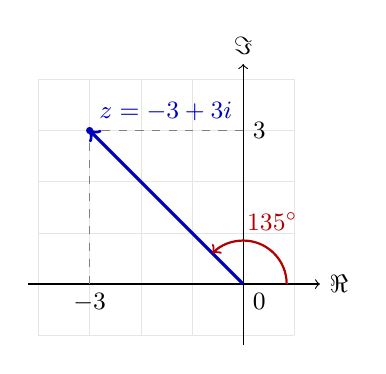
\begin{tikzpicture}[scale=0.65,font=\small]
\draw[step=1,gray!20,very thin] (-4,-1) grid (1,4);
\draw[->] (-4.2,0)--(1.5,0) node[right] {$\Re$};
\draw[->] (0,-1.2)--(0,4.3) node[above] {$\Im$};
\draw[dashed,gray] (-3,0)--(-3,3)--(0,3);
\draw[->,blue!75!black,very thick] (0,0)--(-3,3);
\fill[blue!75!black] (-3,3) circle[radius=2pt] node[above right] {$z=-3+3i$};
\node[below] at (-3,0) {$-3$};
\node[right] at (0,3) {$3$};
\node[below right] at (0,0) {$0$};
\draw[->,red!70!black,thick] (0.85,0) arc[start angle=0,end angle=135,radius=0.85];
\node[red!70!black] at (65:1.35) {$135^\circ$};
\end{tikzpicture}
\end{column}
\begin{column}{0.44\textwidth}
\small
The point $(-3,3)$ lies in \textbf{quadrant II}.
\[
|z|=\sqrt{(-3)^2+3^2}=3\sqrt2.
\]
The reference angle is $45^\circ$, so
\[
\arg(z)=180^\circ-45^\circ=135^\circ.
\]
Using only $\arctan(b/a)$ would give $-45^\circ$, which is the wrong quadrant.
\end{column}
\end{columns}
\end{frame}


\begin{frame}{Drawing a vector and labeling}
  \begin{figure}[h!]
  \centering
    \begin{tikzpicture}[scale=1]
      \draw[->] (-1,0) -- (4,0) node[right]{Re};
      \draw[->] (0,-1) -- (0,3) node[above]{Im};
      \draw[thick,->] (0,0) -- (3,2) node[above, right]{$z=(3,2)$};
      \draw[dashed] (3,0) -- (3,2);
      \node at (1.8,0.2) {3};
      \node at (3.2,1) {2};
      \draw (0.8,0) arc (0:34:0.8) node[midway, left]{$\theta$};
    \end{tikzpicture}
  \end{figure}
\end{frame}

%%%%%%%%%%%%%%%%
\section{Polar Form}
\frame{\sectionpage}
%%%%%%%%%%%%%%%%

\begin{frame}{The cis notation: cosine plus $i$ sine}
\begin{defn}{}{}
For an angle $\theta$, define
\[
\operatorname{cis}\theta=\cos\theta+i\sin\theta.
\]
Throughout this lecture, \textbf{all angles are measured in degrees}.
\end{defn}
For example,
\[
\operatorname{cis}0^\circ=1,\qquad
\operatorname{cis}90^\circ=i,\qquad
\operatorname{cis}180^\circ=-1.
\]
\begin{remark}{A full turn gives the same complex number}
For any integer $k$,
\[
\operatorname{cis}(\theta+360^\circ k)=\operatorname{cis}\theta.
\]
\end{remark}
\end{frame}

\begin{frame}{Polar form $(r,\theta)$}
\begin{defn}{}{}
A complex number $z =a+bi$ can also be expressed in polar form as 
\begin{eq}
z &=& r(\cos\theta + i\sin\theta) \\
&=& r \operatorname{cis}\!\left(\theta\right)
\end{eq} 
where $r=|z|$ is the modulus and $\theta=\arg(z)$ is the argument.
\tcblower
We have
\begin{eq}
a &=& r \cos \theta \\
b &=& r \sin \theta
\end{eq}
\end{defn}
\end{frame}

\begin{frame}{Drawing a vector and labeling}
  \begin{figure}[h!]
  \centering
    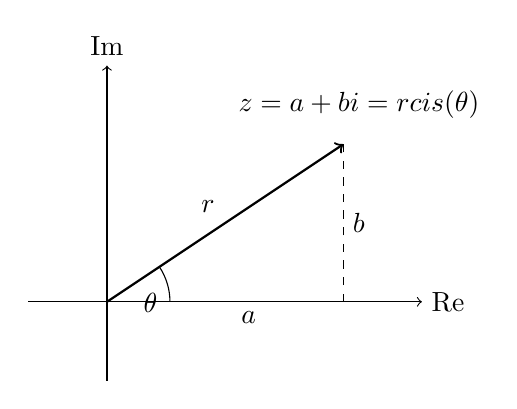
\begin{tikzpicture}[scale=1]
      \draw[->] (-1,0) -- (4,0) node[right]{Re};
      \draw[->] (0,-1) -- (0,3) node[above]{Im};
      \draw[thick,->] (0,0) -- (3,2) node[midway, above left] {$r$}; 
      \node at (3.2,2.5) {$z=a+bi = r\operatorname{cis}\!\left(\theta\right)$};
      \draw[dashed] (3,0) -- (3,2);
      \node at (1.8,-0.2) {$a$};
      \node at (3.2,1) {$b$};
      \draw (0.8,0) arc (0:34:0.8) node[midway, below left]{$\theta$};
    \end{tikzpicture}
    \caption{Representing a complex number both in rectangular form $(a+bi)$ and polar form ($r\operatorname{cis}\!\left(\theta\right)$)}
  \end{figure}
\end{frame}

\begin{frame}[t]
\begin{ex}
Change the following complex numbers in polar form to rectangular form.
\begin{tasks}(3)
\task $4\operatorname{cis}\!\left(30^\circ\right)$
\task $-5\operatorname{cis}\!\left(120^\circ\right)$
\task $\frac{1}{2} \operatorname{cis}\!\left(90^\circ\right)$
\end{tasks}
\end{ex}
\begin{sol}
\begin{tasks}
\task $4\operatorname{cis}\!\left(30^\circ\right) = 4(\cos(30^\circ) + i\sin(30^\circ)) = 4 \left( \frac{\sqrt{3}}{2} + i \frac{1}{2}\right) = 2 \sqrt{3} + 2i$
\task $-5\operatorname{cis}\!\left(120^\circ\right) = -5(\cos(120^\circ) + i\sin(120^\circ)) = -5 \left( -\frac{1}{2} + i \frac{\sqrt{3}}{2}\right) = \frac{5}{2} - \frac{5\sqrt{3}}{2}i$
\task $\frac{1}{2} \operatorname{cis}\!\left(90^\circ\right) = \frac{1}{2} (\cos(90^\circ) + i\sin(90^\circ)) = \frac{1}{2}(i) = \frac{i}{2}$
\end{tasks}
\end{sol}
\end{frame}

\begin{frame}{Multiplication in polar form}
The nice thing about the polar form is that multiplication, division, and powers become easier!
\begin{thm}{}{}
Let $z_1 = r_1 \operatorname{cis}\!\left(\theta_1\right)$ and $z_2 = r_2 \operatorname{cis}\!\left(\theta_2\right)$. Then
\begin{eq}
z_1 z_2 = r_1 r_2 \operatorname{cis}\!\left(\theta_1 + \theta_2\right)
\end{eq}
\end{thm}
Interpretation: to multiply two complex numbers, multiply their lengths and add their angles.
\end{frame}
\begin{frame}{Multiplication: multiply lengths and add angles}
\begin{columns}[c]
\begin{column}{0.55\textwidth}
\centering
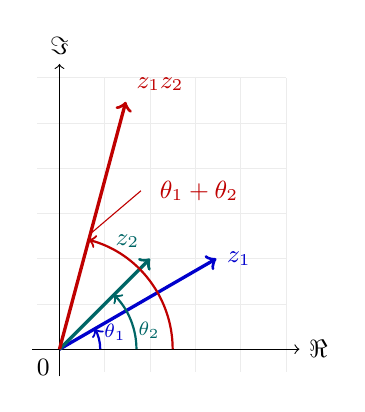
\begin{tikzpicture}[scale=1.15,font=\small]
\draw[step=0.5,gray!15,very thin] (-0.25,-0.25) grid (2.5,3);
\draw[->] (-0.3,0)--(2.65,0) node[right] {$\Re$};
\draw[->] (0,-0.3)--(0,3.15) node[above] {$\Im$};
\node[below left] at (0,0) {$0$};
\draw[->,blue!80!black,very thick] (0,0)--({sqrt(3)},1) node[right] {$z_1$};
\draw[->,teal!80!black,very thick] (0,0)--(1,1) node[above left] {$z_2$};
\draw[->,red!75!black,very thick] (0,0)--({sqrt(3)-1},{sqrt(3)+1}) node[above right] {$z_1z_2$};
\draw[->,blue!80!black,thick] (0.45,0) arc[start angle=0,end angle=30,radius=0.45];
\node[blue!80!black,font=\scriptsize] at (17:0.64) {$\theta_1$};
\draw[->,teal!80!black,thick] (0.85,0) arc[start angle=0,end angle=45,radius=0.85];
\node[teal!80!black,font=\scriptsize] at (12:1.01) {$\theta_2$};
\draw[->,red!75!black,thick] (1.25,0) arc[start angle=0,end angle=75,radius=1.25];
\draw[red!75!black,thin] (75:1.32)--(0.9,1.75);
\node[red!75!black,anchor=west] at (1.0,1.75) {$\theta_1+\theta_2$};
\end{tikzpicture}
\end{column}
\begin{column}{0.42\textwidth}
\small
\textcolor{blue!80!black}{$z_1=\sqrt3+i$}: length $2$, angle $\theta_1=30^\circ$.

\medskip
\textcolor{teal!80!black}{$z_2=1+i$}: length $\sqrt2$, angle $\theta_2=45^\circ$.

\medskip
\textcolor{red!75!black}{$z_1z_2=(\sqrt3-1)+(\sqrt3+1)i$}:
\[
|z_1z_2|=2\sqrt2,
\]
\[
\arg(z_1z_2)=30^\circ+45^\circ=75^\circ.
\]
The three arcs start on the positive real axis.
\end{column}
\end{columns}
\end{frame}


\begin{frame}{Division in polar form}
\begin{thm}{}{}
Let $z_1 = r_1 \operatorname{cis}\!\left(\theta_1\right)$ and $z_2 = r_2 \operatorname{cis}\!\left(\theta_2\right)$. Then
\begin{eq}
\frac{z_1}{z_2} = \frac{r_1}{r_2} \operatorname{cis}\!\left(\theta_1 - \theta_2\right)
\end{eq}
\end{thm}
Interpretation: the denominator must have positive modulus. Divide the lengths and subtract the angles.
\end{frame}
\begin{frame}[t]{Polar division: positive angle difference}
\small
\begin{ex}
Divide $6\operatorname{cis}\!\left(150^\circ\right)$ by $2\operatorname{cis}\!\left(30^\circ\right)$.
\end{ex}
\begin{sol}
\[\frac{6\operatorname{cis}\!\left(150^\circ\right)}{2\operatorname{cis}\!\left(30^\circ\right)}=\frac62\operatorname{cis}\!\left(150^\circ-30^\circ\right)=3\operatorname{cis}\!\left(120^\circ\right).\] Divide the moduli and subtract the denominator angle from the numerator angle.
\end{sol}
\end{frame}

\begin{frame}[t]{Polar division: negative angle difference}
\small
\begin{ex}
Divide $2\operatorname{cis}\!\left(30^\circ\right)$ by $4\operatorname{cis}\!\left(120^\circ\right)$.
\end{ex}
\begin{sol}
\[\frac{2\operatorname{cis}\!\left(30^\circ\right)}{4\operatorname{cis}\!\left(120^\circ\right)}=\frac12\operatorname{cis}\!\left(-90^\circ\right)=-\frac{i}{2}.\] The argument difference is $-90^\circ$, equivalently $270^\circ$; the modulus is positive.
\end{sol}
\end{frame}


\begin{frame}[t]
\begin{ex}
Find the multiplications in polar form.
\begin{tasks}(2)
\task $(3 \operatorname{cis}\!\left(90^\circ\right))(2 \operatorname{cis}\!\left(60^\circ\right))$
\task $(-\operatorname{cis}\!\left(180^\circ\right))\left( \frac{1}{2} \operatorname{cis}\!\left(-90^\circ\right) \right)$
\end{tasks}
\end{ex}
\begin{sol}
\begin{eq*}
(3 \operatorname{cis}\!\left(90^\circ\right))(2 \operatorname{cis}\!\left(60^\circ\right)) &=& (3)(2) \operatorname{cis}\!\left(90^\circ+60^\circ\right) \\
&=& 6 \operatorname{cis}\!\left(150^\circ\right) \\
(-\operatorname{cis}\!\left(180^\circ\right))\left( \frac{1}{2} \operatorname{cis}\!\left(-90^\circ\right) \right) &=& (-1)\left(\frac{1}{2}\right) \operatorname{cis}\!\left(180^\circ+(-90^\circ)\right) \\
&=& -\frac{1}{2}\operatorname{cis}\!\left(90^\circ\right)
\end{eq*}
\end{sol}
\end{frame}

\begin{frame}{Powers: De Moivre's theorem}
Notice that if we multiply repeatedly, we have
\begin{eq*}
(r \operatorname{cis}\!\left(\theta\right))^2 &=& (r \operatorname{cis}\!\left(\theta\right)) (r\operatorname{cis}\!\left(\theta\right)) = r^2 \operatorname{cis}\!\left(2\theta\right) \\
(r \operatorname{cis}\!\left(\theta\right))^3 &=& (r \operatorname{cis}\!\left(\theta\right)) (r \operatorname{cis}\!\left(\theta\right))^2 = r^3 \operatorname{cis}\!\left(3\theta\right).
\end{eq*}
Indeed, this observation is true for any positive power!
\begin{thm}{De Moivre}{}
Let $r$ and $\theta$ be real numbers and $n$ be a positive integer. Then, we have
\begin{equation}
(r \operatorname{cis}\!\left(\theta\right))^n = r^n \operatorname{cis}\!\left(n\theta\right)
\end{equation}
\end{thm}
\end{frame}

\begin{frame}[t]
\begin{ex}
Compute the following powers.
\begin{tasks}(2)
\task $(2\operatorname{cis}\!\left(45^\circ\right))^4$
\task $\left(\frac{1}{3} \operatorname{cis}\!\left(30^\circ\right) \right)^3$
\end{tasks}
\end{ex}
\begin{sol}
\begin{tasks}(1)
\task $(2\operatorname{cis}\!\left(45^\circ\right))^4 = 2^4 \operatorname{cis}\!\left(4 \times 45^\circ\right) = 16\operatorname{cis}\!\left(180^\circ\right)$
\task $\left(\frac{1}{3} \operatorname{cis}\!\left(30^\circ\right) \right)^3 = \left(\frac{1}{3}\right)^3 \operatorname{cis}\!\left(3 \times 30^\circ\right) = \frac{1}{27} \operatorname{cis}\!\left(90^\circ\right)$
\end{tasks}
\end{sol}
\end{frame}


\begin{frame}[t]
\begin{ex}
Find a complex number $z$ such that $z^3 = 125 \operatorname{cis}\!\left(60^\circ\right)$.
\end{ex}
\begin{sol}
If we write $z = r\operatorname{cis}\!\left(\theta\right)$, then $z^3 = r^3 \operatorname{cis}\!\left(3\theta\right)$. We can simply compare
\[r^3 \operatorname{cis}\!\left(3\theta\right) = 125 \operatorname{cis}\!\left(60^\circ\right)\]
so that we have $r^3=125$ and $3\theta = 60^\circ$. These give us $r=5$ and $\theta = 20^\circ$, and thus
\[z = 5 \operatorname{cis}\!\left(20^\circ\right)\]
is a complex number such that $z^3 = 125 \operatorname{cis}\!\left(60^\circ\right)$.
\end{sol}
\end{frame}

\begin{frame}{An n-th root}
In the previous example, we have
\[ z^3 = 125 \operatorname{cis}\!\left(60^\circ\right) \]
and then we can write
\[z = (125 \operatorname{cis}\!\left(60^\circ\right)) ^{\frac{1}{3}}.\]

In particular, we have the following definition:
\begin{defn}{}{}
Let $z$ and $w$ be complex numbers and $n$ be a positive integer such that $z^n = w$. Then we have
\[z = w^{\frac{1}{n}}\]
and call $z$ an $n$-th root of $w$.
\end{defn}
\end{frame}

%%%%%%%%%%%%%%%%
\section[Roots]{Roots of Complex Numbers}
\frame{\sectionpage}
%%%%%%%%%%%%%%%%

\begin{frame}{Roots of unity}
Consider the polynomial
\[x^n = 1\]
where $n$ is a natural number. We know that
\begin{eq*}
x^2=1 &\rightarrow& x = -1,1\\
x^3 = 1 & \rightarrow& x = 1 \\
x^4 = 1 & \rightarrow& x = -1, 1
\end{eq*}
and so on. Note that $x^3=1$ has one real root $x=1$, but the degree of 3 suggests there should be 3 roots in total. Using complex numbers, we can find the other two roots.
\end{frame}

\begin{frame}{}
We rewrite the equation as:
\[x^3 = 1\]
If $x = r\operatorname{cis}\!\left(\theta\right)$, then
\[x^3= r^3\operatorname{cis}\!\left(3\theta\right)\]

We see that $r=1$ since the modulus (or length) of the right-hand side is 1. However, $\theta$ requires attention because note that
\[1 = \operatorname{cis}\!\left(0^\circ\right)\]
and setting $3\theta = 0^\circ$ gives us $\theta = 0^\circ$ as one solution. But actually, using trigonometry we have
\[1 = \operatorname{cis}\!\left(360^\circ k\right) \]
where $k$ is an integer. This means that we can rotate the complex number $360$ degrees and return to the same point. Thus, the correct equation is:
\[3 \theta = 360^\circ k \]
\end{frame}

\begin{frame}{}
Finally, we have:
\begin{eq*}
(k=0) \quad 3\theta = 0^\circ &\rightarrow& \theta = 0^\circ \\
(k=1) \quad 3\theta = 360^\circ & \rightarrow& \theta = 120^\circ \\
(k=2) \quad 3\theta = 720^\circ & \rightarrow& \theta = 240^\circ \\
(k=3) \quad 3\theta = 1080^\circ & \rightarrow& \theta = 360^\circ
\end{eq*}
Since $\theta = 0^\circ$ and $\theta = 360^\circ$ are the same angle, they yield the same solution. Thus, the roots of the polynomial $x^3=1$ are:
\[x = 1, \; \operatorname{cis}\!\left(120^\circ\right), \; \operatorname{cis}\!\left(240^\circ\right),\]
or in rectangular form $a+bi$: $1, \; -\frac{1}{2} + \frac{\sqrt{3}}{2}i, \; -\frac{1}{2} - \frac{\sqrt{3}}{2}i$.
\end{frame}

\begin{frame}{Roots of Unity}
\begin{thm}{}{}
The roots of $x^n=1$ where $n$ is a natural number are
\begin{equation}
x = \operatorname{cis}\!\left(\frac{360^\circ k}{n}\right), \quad k=0,1,2,\ldots,n-1
\end{equation}
These are called ``roots of unity'' of degree $n$. Geometrically, these are unit vectors equally spaced around the origin.
\end{thm}
\end{frame}

\begin{frame}[t]
\begin{figure}[h!]
\centering
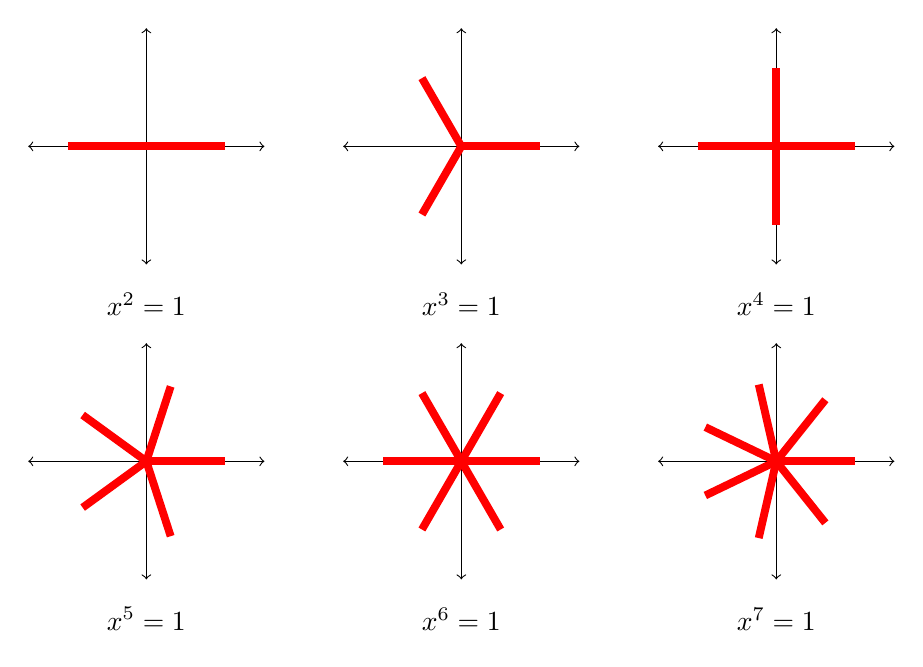
\begin{tikzpicture}
\foreach \n / \x / \y in {2/1/1,3/2/1,4/3/1,5/1/2,6/2/2,7/3/2} {
	\begin{scope}[xshift = {4*\x cm}, yshift={-4*\y cm}] 
		\draw[<->] (-1.5,0)--(1.5,0);
		\draw[<->] (0,-1.5)--(0,1.5);
		\foreach \k in {0,1,...,\n} {
			\draw[line width = 0.1cm, red] (0,0) -- ({\k*360/\n}:1cm);
		}
		\node at (0, -2) {$x^{\n} = 1$};
	\end{scope}
}
\end{tikzpicture}
\caption{Roots of unity for different values of $n$}
\end{figure}
\end{frame}

\begin{frame}[t]
\begin{ex}
Find the roots of unity of degree 4.
\end{ex}
\begin{sol}
Applying the theorem, the roots are
\[x = \operatorname{cis}\!\left(\frac{360^\circ k}{4}\right), \quad k=0,1,2,3\]
These are $\operatorname{cis}\!\left(0^\circ\right), \operatorname{cis}\!\left(90^\circ\right), \operatorname{cis}\!\left(180^\circ\right), \operatorname{cis}\!\left(270^\circ\right)$, which can also be expressed as $1, i, -1, -i$.
\end{sol}
\end{frame}
\begin{frame}[t]{Roots of unity: degree six}
\small
\begin{ex}
Find all solutions of $z^6=1$ using the roots-of-unity formula.
\end{ex}
\begin{sol}
Using degree angles,\[z_k=\operatorname{cis}\!\left(60^\circ k\right),\quad k=0,1,2,3,4,5.\] The arguments are $0^\circ,60^\circ,120^\circ,180^\circ,240^\circ,300^\circ$. Each root has modulus $1$. Its sixth power has argument a multiple of $360^\circ$, so equals $1$.
\end{sol}
\end{frame}



\begin{frame}{N-th roots}
For any complex number $z = r\operatorname{cis}\!\left(\theta\right)$, recall that we can find an $n$-th root using De Moivre's rule:
\[ z^{\frac{1}{n}} = r^{\frac{1}{n}} \operatorname{cis}\!\left(\frac{\theta}{n}\right)\]
Now, we can find \textbf{all} $n$-th roots using roots of unity.
\begin{thm}{}{}
Let $z=r\operatorname{cis}\!\left(\theta\right)$ be a complex number and $n$ be a natural number. The $n$-th roots of $z$ are
\begin{equation}
z_k = r^{\frac{1}{n}} \operatorname{cis}\!\left(\frac{\theta + 360^\circ k}{n}\right), \quad k=0,1,2,\ldots,n-1
\end{equation}
We have $z_k^n = z$.
\end{thm}
\end{frame}

\begin{frame}[t]
\begin{ex}
Find all cube roots of 8.
\end{ex}
\begin{sol}
Write $8 = 8 \operatorname{cis}\!\left(0^\circ\right)$. Cube roots are:
\[ 8^{1/3} \operatorname{cis}\!\left(\frac{0^\circ + 360^\circ k}{3}\right) = 2 \operatorname{cis}\!\left(120^\circ k\right),\quad k=0,1,2. \]
These are: $2,\; 2\operatorname{cis}\!\left(120^\circ\right)$ and $\; 2\operatorname{cis}\!\left(240^\circ\right).$
\end{sol}
\end{frame}

\begin{frame}[t]
\begin{ex}
Find all fourth roots of -81.
\end{ex}
\begin{sol}
Write $-81 = 81 \operatorname{cis}\!\left(180^\circ\right)$. Fourth roots are:
\[ 81^{1/4} \operatorname{cis}\!\left(\frac{180^\circ + 360^\circ k}{4}\right) = 3 \operatorname{cis}\!\left(45^\circ + 90^\circ k\right),\quad k=0,1,2,3. \]
These are: $3 \operatorname{cis}\!\left(45^\circ\right), 3\operatorname{cis}\!\left(135^\circ\right), 3\operatorname{cis}\!\left(225^\circ\right)$ and $3\operatorname{cis}\!\left(315^\circ\right).$
\end{sol}
\end{frame}